\section{Acquisizione dati}
Una volta montato ogni circuito, come nell'esperienza precedente, è stato collegato l'oscilloscopio sia direttamente al generatore di forme d'onda sia al circuito in analisi. 
\`E stata fissata anche questa volta una tensione a $1\,Vpp$ e, dopo aver stabilizzato con il comando $trigger$ le forme d'onda sullo schermo e averle allineate, sono state impostate le funzioni integrate dell'oscilloscopio che permettevano di ottenere direttamente a schermo i valori di picco dei due segnali e di differenza di fase tra i medesimi.\phantom{maperchédevosempreognivoltamettereapostolecoseconunphantom?melospieghi?chestoria!}\begin{wrapfigure}[26]{r}[0pt]{100mm}
%	\centering
    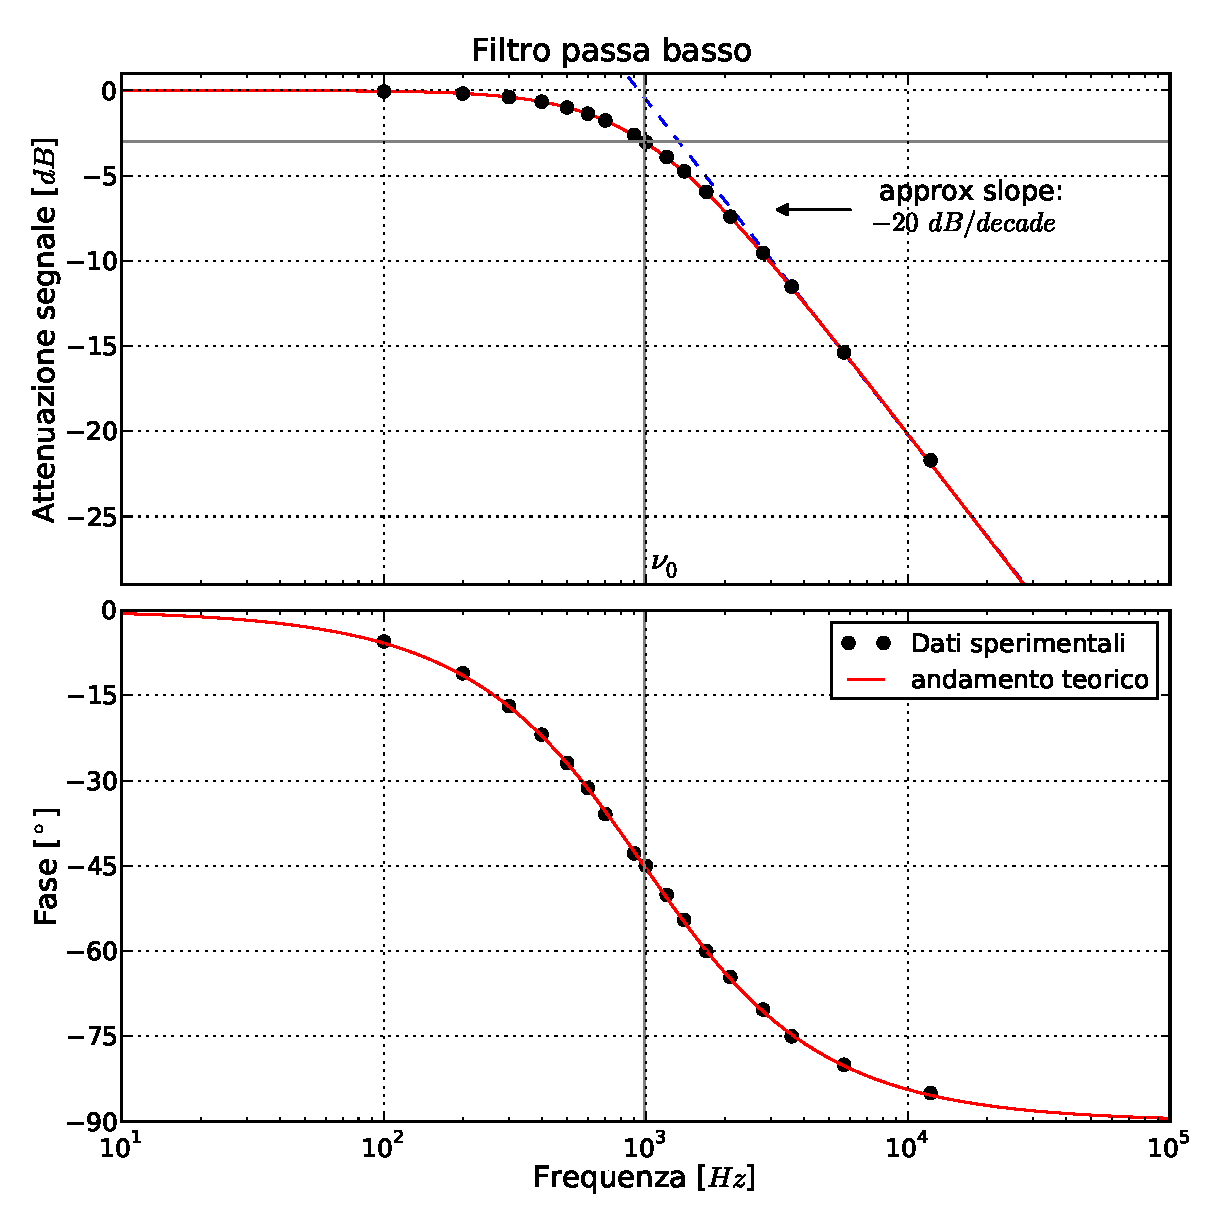
\includegraphics[width=105mm]{low.pdf}
    \caption{Diagrammi di Bode per il filtro passa basso.}
    \label{fig:low}
\end{wrapfigure}

\section{Passa basso}

Per quanto riguarda il filtro passa basso abbiamo scelto di prendere misure di tensione e differenza di fase circa ogni $5^{\circ}$, sapendo a priori che nei diagrammi di Bode l'unico valore non graficato con un logaritmo sarebbe stata la fase $\phi$.

Come mostrato in Fig.\ref{fig:circuito}, il filtro passa basso è composto da una resistenza e da un condensatore. Intuitivamente, poichè il condensatore si comporta come un filo ideale per alte frequenze mentre come circuito aperto per le basse, si vede immediatamente che per frequenze alte i due capi dell'oscilloscopio si troveranno cortocircuitati tra loro. Dunque tale filtro farà passare le frequenze basse.

Quantitativamente, utilizzando la legge di Ohm generalizzata ($V=Z \cdot I$), ovvero introducendo il concetto di impedenze, è possibile trattare tale circuito come un partitore generalizzato. Risulta dunque semplice trovare il valore di tensione ai capi del condensatore in funzione della frequenza in input nel circuito. Una volta determinata tale funzione, è possibile calcolare il rapporto tra valore picco-picco di $V_{out}$ con $V_{in}$. \`E anche semplice ricavare la differenza di fase con il segnale in input, utilizzando la formula $\phi=arctan[\frac{Im(V_{out})}{Re(V_{out})}]$. Riportiamo le equazioni da noi calcolate analiticamente, ricordando che $Z_R=R$ e $Z_C=-\frac{j}{\omega C}$.\\

\noindent
\begin{minipage}{.5\linewidth}
\begin{equation}
\frac{|V_{out}|}{|V_{in}|}=
\label{eq:lowGain}
\end{equation}

\end{minipage}%
\begin{minipage}{.5\linewidth}
\begin{equation}
\phi=arctan[3.6]
\label{eq:lowPhi}
\end{equation}
\end{minipage}
\break

I valori delle componenti circuitali utilizzate sono $R=(8746 \pm 53)\,\si{\ohm}$ e $C=(73+6 \pm 213)\,\si{\nano\farad}$.

Il diagramma di Bode\footnote{Un diagramma di Bode è una rappresentazione grafica della risposta in frequenza di un circuito e che consiste in due grafici che rappresentano rispettivamente l'ampiezza e la fase della funzione complessa di risposta in frequenza. In entrambi i grafici l'asse delle ascisse è logaritmica, mentre in quella delle ordinate vengono riportate rispettivamente il guadagno di segnale (in $\si{\decibel}$) e la fase (in gradi o radianti)} in Fig. \ref{fig:low} riporta i valori acquisiti per il filtro passa basso. Nel caso di questo filtro, si definisce una frequenza, detta di taglio, ($\nu_{taglio}=\frac{1}{2 \pi RC}$) tale per cui il rapporto fra l'ampiezza\footnote{la scala in decibel per la potenza è definita diversamente} dei segnali uscente ed entrante valga $\frac{|V_{out}|}{|V_{in}|}\,=\,\frac{\sqrt{2}}{2}\,=\,\frac{1}{\sqrt{2}}$. Si osserva che in questo caso il valore di guadagno vale $20Log(\frac{|V_{out}|}{|V_{in}|})\,=\,-3\,\si{\decibel}$ e quello di fase $\phi=-45 ^{\circ}$. Come si vede in Fig. \ref{fig:low} tale previsione teorica è confermata dai dati sperimentali.

Inoltre, nel primo diagramma, osserviamo che per valori di frequenza maggiori di quella di taglio l'attenuazione tende asintoticamente ad una retta. In base alla pendenza di tale retta, che nel nostro caso è di $-\textbf{??}\frac{\si{\decibel}}{decade}$, si definisce il \emph{fattore di bontà} del filtro passa-basso.

Notiamo infine come leggi teoriche sopra calcolate e dati sperimentali siano compatibili tra loro.
%
\begin{wrapfigure}[28]{r}[0pt]{100mm}
%	\centering
    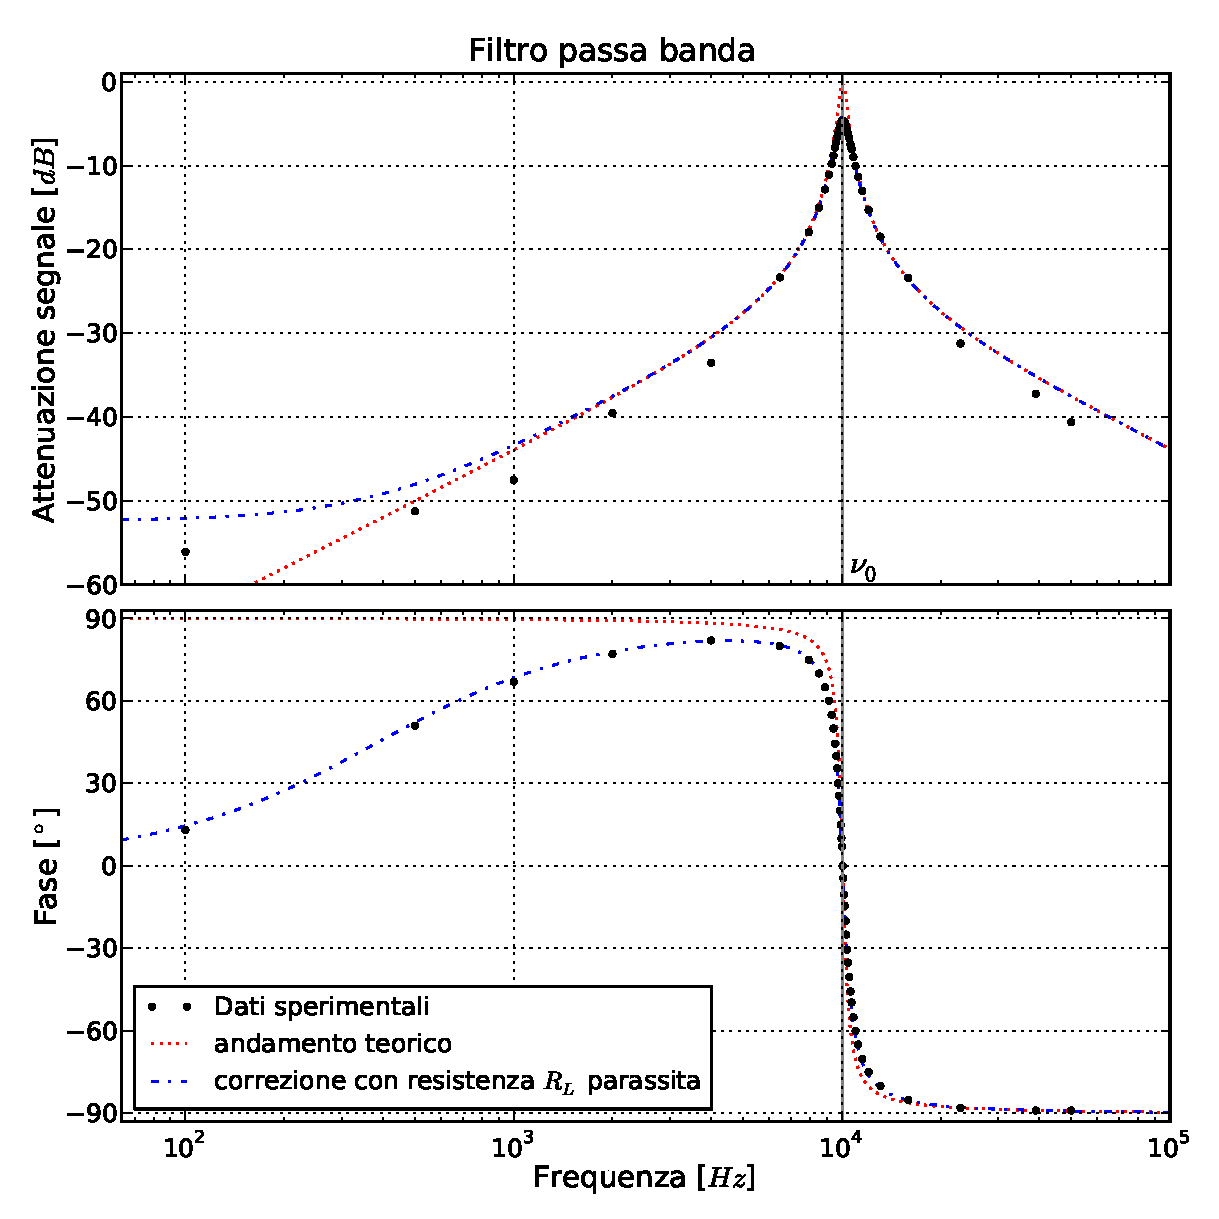
\includegraphics[width=105mm]{bpf.pdf}
    \caption{Diagrammi di Bode per il filtro passa banda.}
    \label{fig:bpf}
\end{wrapfigure}

\section{Passa banda}
Questo secondo filtro analizzato, oltre che resistenza e condensatore, prevede l'utilizzo di un'induttanza. In Fig. \ref{fig:circuito} è rappresentato il circuito utilizzato. Il parallelo di induttanza e condensatore fa si che sia per frequenze basse che per quelle alte l'oscilloscopio sia cortocircuitato. Infatti l'induttanza si comporta come filo ideale per frequenze basse mentre come circuito aperto per quelle alte. Tale filtro lascerà passare dunque solo un range di frequenze attorno al valore $\nu_0$, detta frequenza di risonanza e definita come $\nu_0=\frac{1}{2 \pi \sqrt{LC}}$. Per questo motivo abbiamo deciso di prendere misure circa ogni $5^\circ$ a salire e a scendere in frequenza partendo da $\nu_0$.

Come fatto nel paragrafo precedente, è possibile utilizzare il concetto di partitore generalizzato per risolvere il circuito. Ricordiamo che l'induttanza ha una impedenza $Z_L=j\omega L$. Ricaviamo pertanto le seguenti leggi:

%\noindent
%\begin{minipage}{.5\linewidth}
\begin{equation}
\frac{|V_{out}|}{|V_{in}|}=
\label{eq:bpfGain}
\end{equation}

%\end{minipage}%
%\begin{minipage}{.5\linewidth}
\begin{equation}
\phi=arctan[3.6]
\label{eq:bpfPhi}
\end{equation}
%\end{minipage}
%\break

I valori delle componenti circuitali utilizzate sono $R=(8746 \pm 53)\,\si{\ohm}$ , $C=(73+6 \pm 213)\,\si{\nano\farad}$ e $L=(weraas54 \pm 864)\,\si{\henry}$.

Come vediamo dal diagramma di Bode, sebbene i dati sperimentali riguardanti la fase siano compatibili con i valori teorici, non possiamo dire lo stesso per l'attenuazione di segnale. Sembra dunque sia stato trascurato qualche effetto parassita. Sicuramente non si tratta di elementi attivi (induttanze o capacità parassite) in quanto esse produrrebbero un uno sfasamento del segnale oltre che un'attenuazione dell'ampiezza di segnale (infatti hanno componente complessa). E' dunque probabile sia stata trascurata qualche resistenza nelle componenti circuitali. Fortunatamente abbiamo misurato la resistenza dell'induttanza, ottendendo come valore $(R_L=2.41\pm 0.01) \Omega$. Inserendo dunque tale resistenza in serie all'induttanza e risolvendo analiticamente il circuito, troviamo delle nuove equazioni (che non riportiamo analiticamente per ragioni di spazio). Nel grafico è possibile apprezzare le correzioni che tale soluzione produce.

\section{Reiezione di Banda o Notch}
L'ultimo filtro analizzato, e quello che più ci ha dato filo da torcere nell'analisi, è stato quello a reiezione di banda.

La struttura del filtro notch, riportata in Fig. \ref{fig:circuito}, attenua l'ampiezza di segnale solo per una determinata frequenza, detta anche in questo caso di risonanza ($\nu_0=\frac{1}{2 \pi \sqrt{LC}}$), alla quale la serie di capacità e induttanza avrà impedenza complessiva nulla. Considerando come valori di $R$, $L$ e $C$ le stesse del circuito passa banda, riportiamo le leggi teoriche calcolate:\\

\noindent
\begin{minipage}{.5\linewidth}
\begin{equation}
\frac{|V_{out}|}{|V_{in}|}=
\end{equation}
\end{minipage}%
\begin{minipage}{.5\linewidth}
\begin{equation}
\phi=arctan[3.6]
\end{equation}
\end{minipage}
\break
\begin{wrapfigure}[28]{r}[0pt]{100mm}
%	\centering
    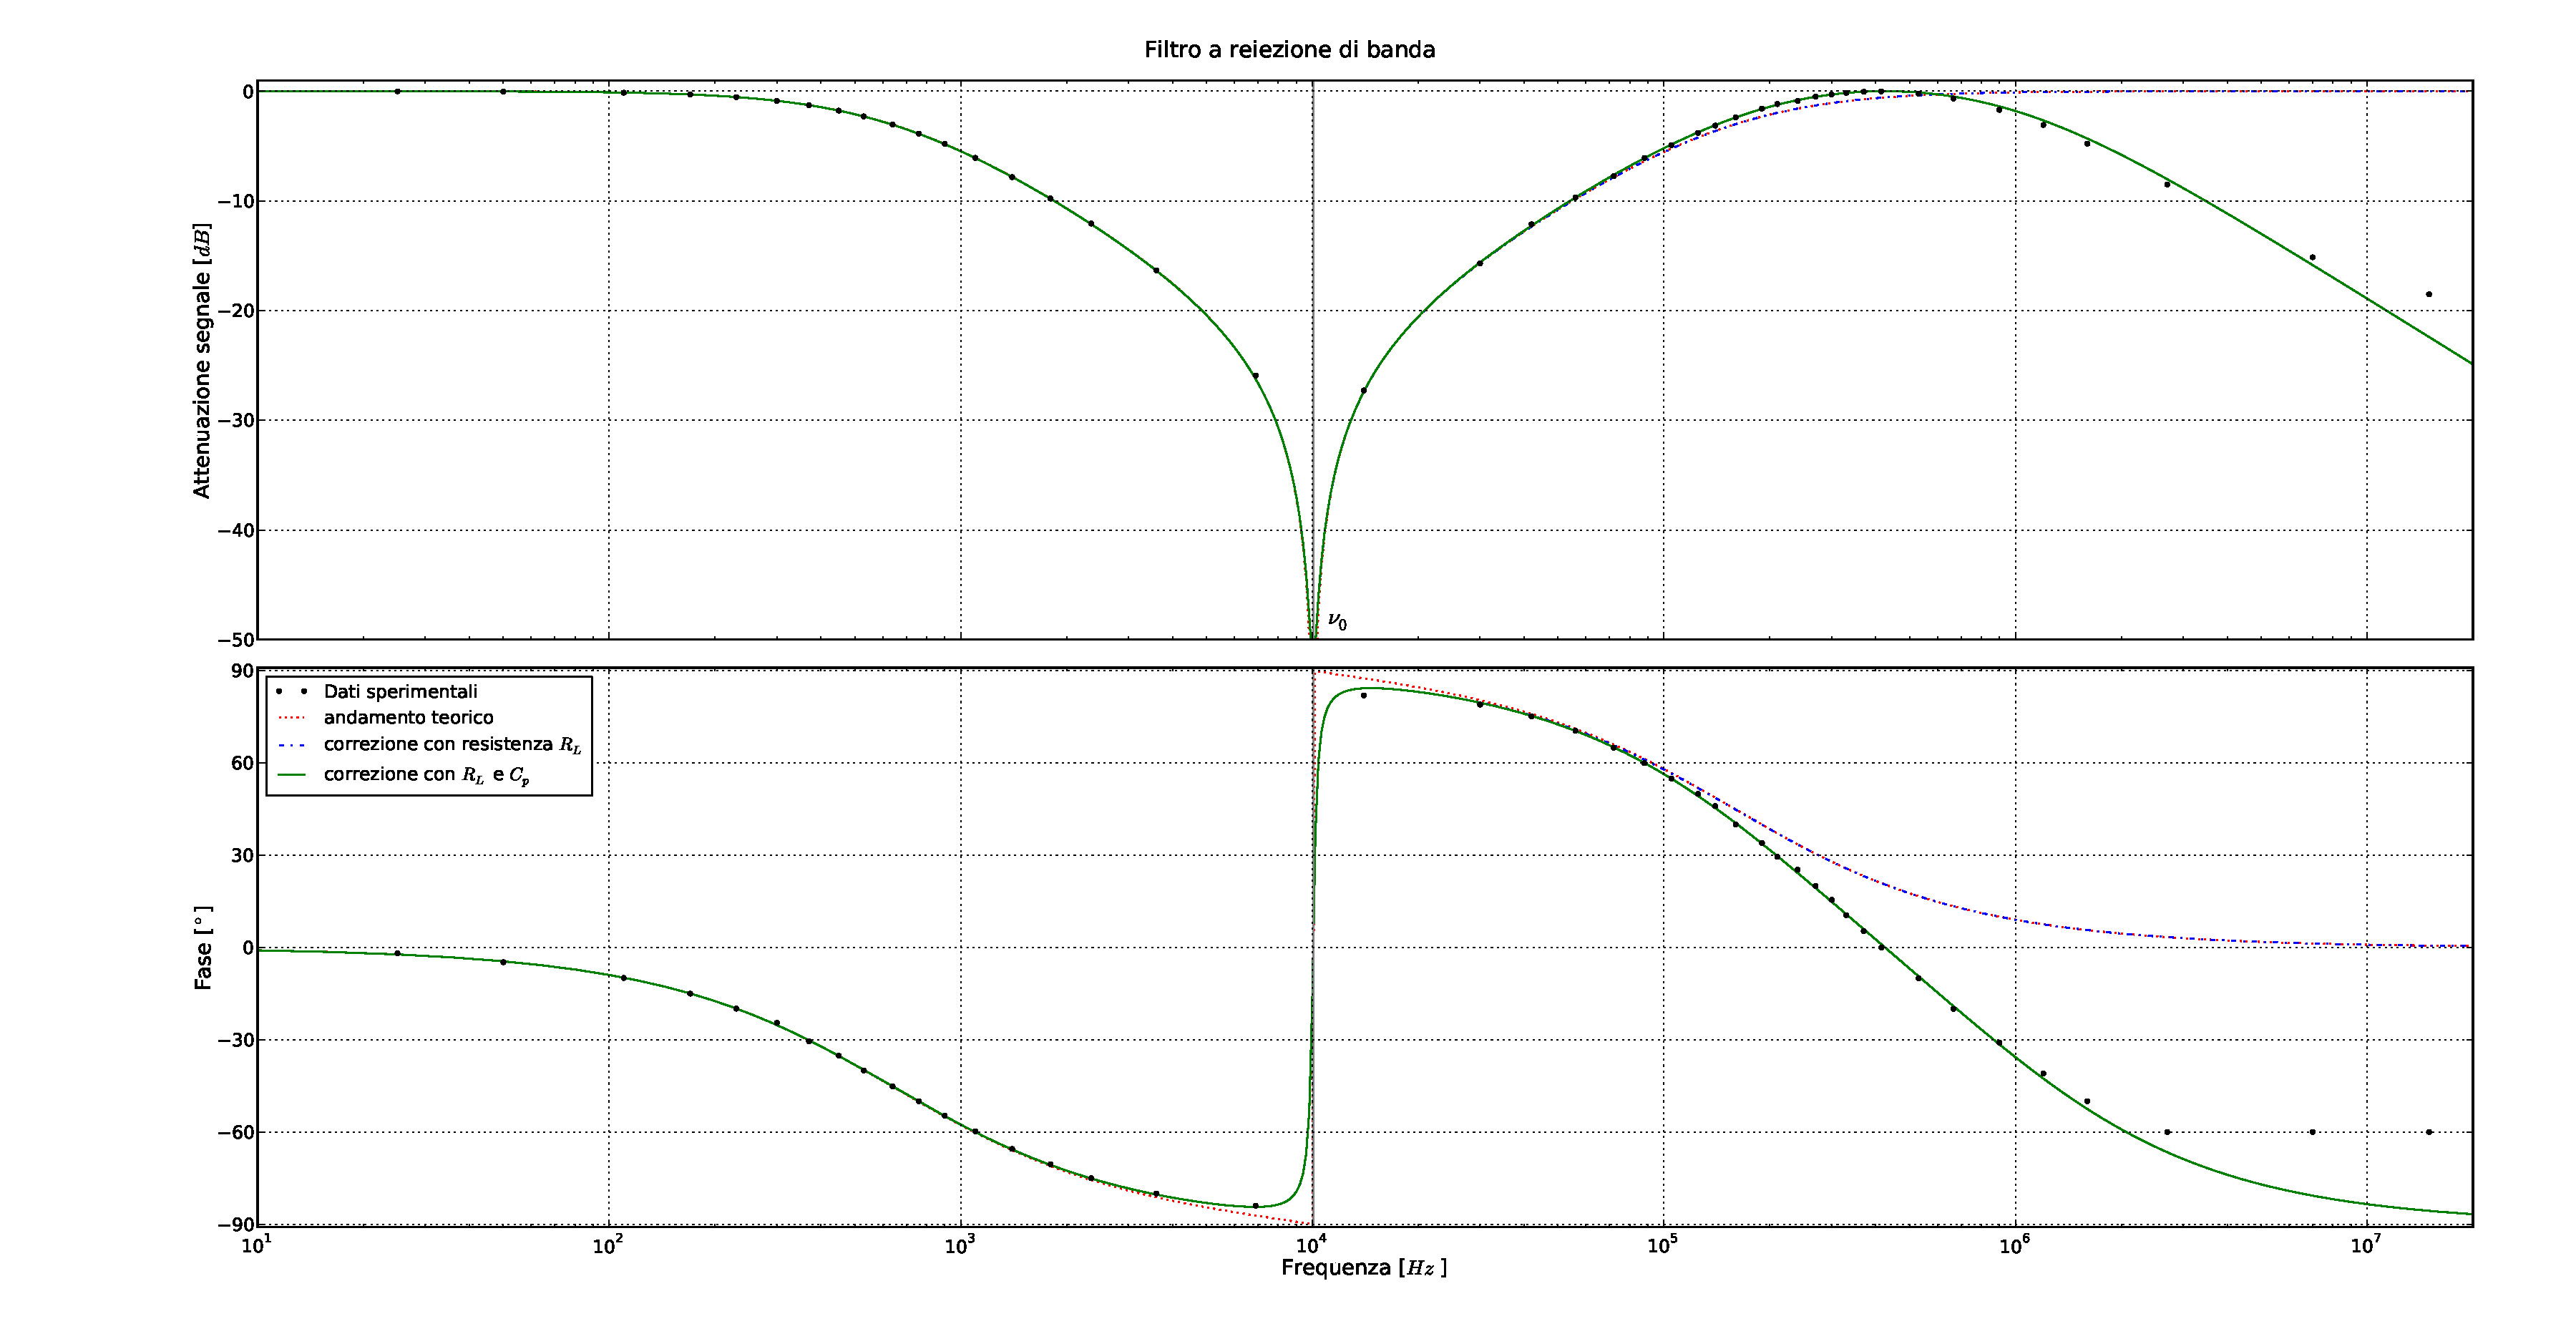
\includegraphics[width=105mm]{notch.pdf}
    \caption{Diagrammi di Bode per il filtro a reiezione di banda.}
    \label{fig:notch}
\end{wrapfigure}

Come osserviamo dal diagramma di Bode per questo circuito, la legge teorica non è compatibile per alte frequenze in nessuno dei due grafici. I dati sembrano infatti seguire una legge ben diversa da quella stimata. Pertanto inizialmente abbiamo risolto analiticamente il circuito considerando anche la resistenza parassita interna all'induttanza. La legge ricavata ha ridotto la discrepanza tra previsione teorica e dati sperimentali solo per le frequenze vicine a $\nu_0$, ma non ad alte frequenze.

Abbiamo dunque cercato un motivo di tale incompatibilità. Dai dati sembra che per alte frequenze ci sia qualcosa che smorza l'intensità del segnale e ne cambia la fase. Abbiamo dunque avanzato varie ipotesi.

Poiché il comportamento ad alte frequenze è simile a quello del filtro passa basso, la prima ipotesi da noi considerata è stata l'\emph{effetto pelle}. Tale fenomeno si presenta in maniera visibile per lo più ad alte frequenze e consiste nel fatto che la corrente tende a scorrere con più facilità sulla superficie del conduttore (ricordiamo che in regime quasi stazionario la corrente scorre uniformemente all'interno di un conduttore omogeneo e isotropo) che al centro del conduttore. Tale effetto potrebbe causare una capacità parassita. Tuttavia, provando ad aggiungere condensatori in serie al circuito, abbiamo visto subito che essi non causerebbero modifiche nella legge teorica per alte frequenze. Abbiamo dunque escluso l'effetto pelle.

Come seconda ipotesi abbiamo le induttanze parassite dei fili. Infatti, come è noto, ogni filo ho una propria induttanza. Abbiamo dunque risolto nuovamente il circuito mettendo un'induttanza subito prima della resistenza e poi, eseguendo vari plot per diversi valori di induttanza parassita, ne abbiamo analizzato l'andamento. Anche in questo caso l'analisi ha dato esito negativo. Tale correzione infatti non porta un miglioramento di compatibilità con i dati da noi raccolti.

Non sappiamo dunque ancora quale sia la causa di tale discrepanza.